\section{Adaptive gradient clipping in \tuner}
\label{sec:adapt_clip}
\begin{figure}
%	%\begin{minipage}{0.61\textwidth}
\centering
%% \vspace{-2.25em}
  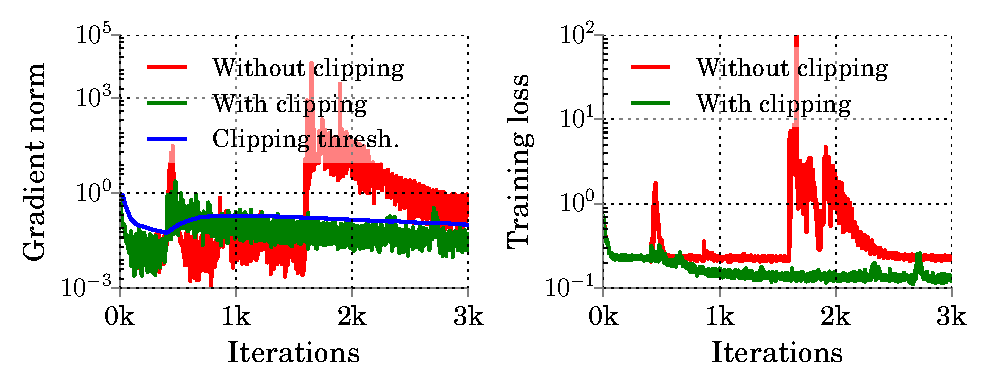
\includegraphics[width=0.7\linewidth]{experiment_results/clipping_example.pdf} 
% \vspace{-0.75em}
\caption{A variation of the LSTM architecture in \citep{zhu2016trained} exhibits exploding gradients.
The proposed adaptive gradient clipping threshold (blue) stabilizes the training loss.}
\label{fig:stability}
%\end{minipage}
\end{figure}

Gradient clipping has been established in literature as a standard---almost necessary---tool for training such objectives \citep{pascanu2013difficulty,Goodfellow-et-al-2016,gehring2017convolutional}. 
However, the classic tradeoff between adaptivity and stability applies: 
setting a clipping threshold that is too low can hurt performance;
setting it to be high, can compromise stability.
\tuner, keeps running estimates of extremal gradient magnitude squares, $h_{max}$ and $h_{min}$ in order to estimate a generalized condition number.
We posit that $\sqrt{h_{max}}$ is an ideal gradient norm threshold for adaptive clipping.
In order to ensure robustness to extreme gradient spikes, like the ones in Figure~\ref{fig:stability}, we also limit the growth rate of the envelope $h_{max}$ in Algorithm~\ref{alg:curv_func} as follows:
\begin{equation}
 h_{max} 
 \leftarrow
 \beta \cdot h_{max}
 	+ (1-\beta) \cdot \textrm{min}\left\{
 		h_{max,t}, 100 \cdot h_{max}
 	\right\}
\end{equation}
Our heuristics follows along the lines of classic recipes like~\cite{pascanu2013difficulty}. However, instead of using the average gradient norm to clip, it uses a running estimate of the maximum norm $h_{\max}$.

In Section~\ref{sec:stability}, we saw that adaptive clipping stabilizes the training on objectives that exhibit exploding gradients. In Figure~\ref{fig:infl_clip}, we demonstrate that the adaptive clipping does not hurt performance on models that do not exhibit instabilities without clipping. Specifically, for both PTB LSTM and CIFAR10 ResNet, the difference between \tuner with and without adaptive clipping diminishes quickly.  
\label{sec:infl_clip}
\begin{figure}
\centering
\begin{tabular}{c c}
	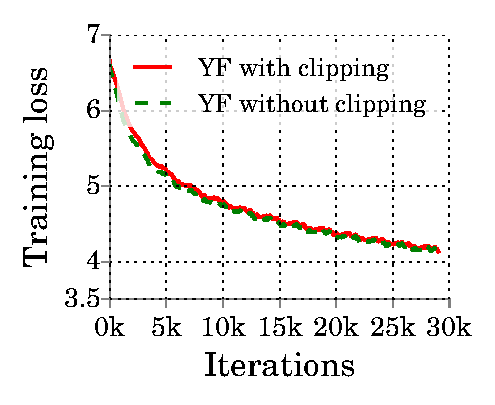
\includegraphics[width=0.35\linewidth]{experiment_results/ptb/clip_cmp.pdf} &
	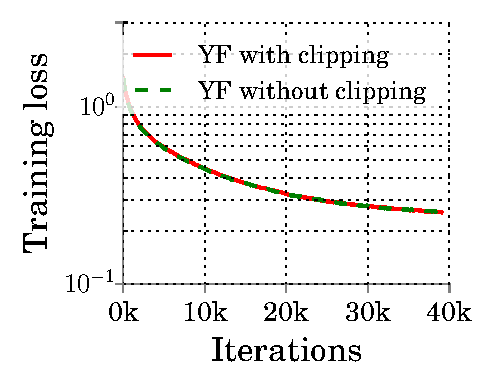
\includegraphics[width=0.35\linewidth]{experiment_results/resnet/cifar10_clip_cmp.pdf}
\end{tabular}
\caption{Training losses on PTB LSTM (left) and CIFAR10 ResNet (right) for YellowFin with and without adaptive clipping.}
\label{fig:infl_clip}
\end{figure}
